\chapter{Preliminaries}
\label{chap:preliminaries}
In this chapter we give a brief introduction to relational-database
normalization. The chapter is intended to be used only as quick reference,
since discussing the relational data model and the relational-database normalization
in detail is beyond the scope of this report. For readers who would like to read
more on the subject we recommend the textbook by Elmasri and Navathe~\cite{bdb1} or
the textbook by Kemper and Eickler~\cite{bdb2} for German-speaking readers, both of which have 
proven to be helpful guides throughout the development process of LDBN. There are also
many free on-line resources such as the article 
\textit{A Simple Guide to Five Normal Forms in Relational Database Theory}
by Kent~\cite{p7}.  

\section{Definitions}
In the following we give some very important definitions to some key
concepts in the relational-database
normalization, such as relation, key, functional dependency, lossless-join, 
2NF, 3NF, BCNF and others. We also provide the reader with examples to illustrate the 
different normalization concepts in practice. We follow the notations 
of Kemper and Eickler~\cite{bdb2}.
All of the following definitions excluding the examples are also taken from~\cite[Chapter 6]{bdb2}.  

\subsection{Relation}
In relational databases data are represented in tables/relations. 
The columns in the table/relation identify the attributes, for instance
in a table for storing personal data of students such attributes could be
name, date of birth and so forth. A row or a tuple contains all the data of a single 
instance of the table such as a student named John Doe.
In the relational model, every row must have a unique identification or 
key based on the data. Figure~\ref{fig:rmodel} shows an example of a relation in which 
the Attribute \textit{Matriculation Number} is the key that uniquely identifies each row/tuple in the relation.

\begin{figure}[h]
  \begin{center}
    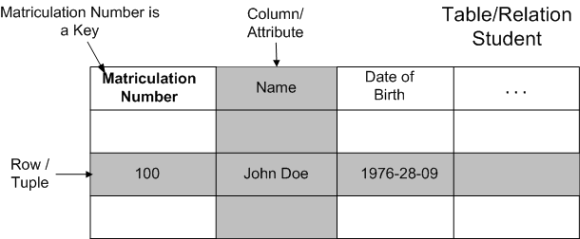
\includegraphics[width=0.85\textwidth]{./img/rmodel01.png}
    \caption{Relation Example}
    \label{fig:rmodel}
  \end{center}
\end{figure}

We would like to give some more formal definitions as well:
\begin{description}
  \item[Relation Schema:] A relation schema is given by a name $R$, together with a finite set
    $Attr(R)$ of attributes. For convenience, when no confusion can result, $R$ will be used as an
    abbreviation for $Attr(R)$.
  \item[Domain:] With each attribute $A \in Attr(R)$ is associated a domain $Dom(A)$, that is
    the set of allowed values for each attribute. 
  \item[Tuple:] A tuple over $R$ is a function $t$ on $Attr(R)$ such that $t(A) \in Dom(A)$
    for each $A \in Attr(A)$. For $\mathbf{B} \subseteq Attr(A)$, the projection of the tuple $t$
    onto $\mathbf{B}$ is is the function $t$ restricted to $\mathbf{B}$.  This
    projection often denoted $t.\mathbf{B}$.  For $\mathbf{B}$ a singleton;
    i.e., $\mathbf{B}=\{C\}$, $t.C$ denotes $t.\{C\}$.
  \item[Relation Instance:] A relation instance $r$ for a relation schema is a set
    of tuples over its attribute set.
  \item[Projection:] Projection is a unary operation written as $\Pi_{\mathbf{B}} (r)$ 
    where $\mathbf{B} \subseteq Attr(A)$  and $r$ is an instance of $R$. 
    $\Pi_{\mathbf{B}} (r) = \{t.\mathbf{B} | t \in r\}$. In words, it deletes attributes that are not in $\mathbf{B}$. 
    Note that duplicate tuples are automatically eliminated by definition.
  \item[Natural Join:] Natural join is a binary operator that is written as $(r \Join s)$ where $r$ and $s$ are relation instances. 
    The result of the natural join is the set of all combinations of tuples in $r$ and $s$ that are equal on their common attribute names.
\end{description}

Subsets of $Attr(A)$ are often written using concatenation, when no
confusion can result.  Thus, if $Attr(A) = \{A,B,C,D\}$, then $\{A,B,C\}$ may
also be written $ABC$. In the following we often use lower-case Greek letters such as
$\alpha$, $\beta$ and $\gamma$ to refer to subset of $Attr(A)$.

\subsection{Key}
As we mentioned a key is used to uniquely identify a tuple. Each table can contain
more than one key. For example,
in our \textit{Student} relation we could also have an attribute \textit{Personal Number} 
which could also be used
as a key. Furthermore, each key may be composed from more than one attribute, for instance, 
all the attributes of every relation always build a key. However, such a key can often be reduced
to a smaller subset of the relation's attributes. 
We refer to keys that cannot be reduces any more without losing their key property as candidate keys.
In addition, each relation has a primary key, which is a selected candidate key for that relation.

\subsection{Functional Dependency}
The concept of Functional Dependency (FD) is central to normalization theory. 
FD is a semantic concept which describes a particular semantic relationship 
between the attributes of a relation. An FD is often represented as $\alpha$ $\rightarrow$ $\beta$, 
where $\alpha$ and $\beta$ are subsets of the attributes of a given relation \textit{R}.
We often refer to $\alpha$ as the left-hand side (LHS) of the FD and to $\beta$ as the 
right-hand side (RHS) of the FD.
The representation $\alpha$ $\rightarrow$ $\beta$ means that for $\beta$ is 
functionally dependent on $\alpha$; that is, for each
for each value of $\alpha$ no more than one value of $\beta$ is associated. 
More formally, if $t$ and $r$ are two tuples in the relation \textit{R}
with $t.\alpha = r.\alpha$ then $t.\beta = r.\beta$. Here
$t.\alpha = r.\alpha$ is a short form for 
\begin{math} \forall A \in \alpha : t.A = r.A \end{math}.  
In other words, the values of the attributes  in $\alpha$ uniquely 
determines the values of of the attributes in $\beta$ and 
if there were several tuples that had the same value of $\alpha$ then all these 
tuples will have identical values for the attributes in $\beta$. 

We would like to illustrate this very important concept of FDs with an example. 
Let us consider the following relation $R = \{A, B, C, D\}$. 
The example comes from~\cite[Section 6.1]{bdb2}.

\begin{center}
\begin{tabular}[h]{l|l|l|l|l|}
  \cline{2-5}
  & \multicolumn{4}{|c|}{$R$} \\ \cline{2-5}
  & $A$ & $B$ & $C$ & $D$ \\ \cline{2-5}
  $t$ & $a_4$ & $b_2$ & $c_4$ & $d_3$ \\ 
  $p$ & $a_1$ & $b_1$ & $c_1$ & $d_1$ \\ 
  $q$ & $a_1$ & $b_1$ & $c_1$ & $d_2$ \\ 
  $r$ & $a_2$ & $b_2$ & $c_3$ & $d_2$ \\ 
  $s$ & $a_3$ & $b_2$ & $c_4$ & $d_3$ \\ \cline{2-5}
\end{tabular}
\end{center}

In this instance $A \rightarrow B$  is satisfied.
As all tuples that have the same A value have the same $B$ value. However,
$B \rightarrow A$ is \textbf{not} satisfied, since the tuples $r$ and $s$ with $r.B = s.B$ have
different $A$ values. Other FDs on the relation which are also satisfied are
$A \rightarrow C$ and $CD \rightarrow B$.

A functional dependency is \textit{trivial} if it satisfied by all tuples, i.e., $\alpha$ $\rightarrow$ $\alpha$.
In general, a functional dependency of the form $\alpha$ $\rightarrow$ $\beta$ is trivial if 
$\beta \subseteq \alpha$.

\subsection{Closure of a Set of FDs}
\label{sec:closureF}
In a relation schema $R$ constrained by a set $F$ of FDs we define the closure of $F$, denoted $F\sp{+}$,
as a set of all possible FDs which can be derived from the original set of FDs $F$. In 
other words, $F\sp{+}$ is the set of all FDs that must always hold in $R$. $F\sp{+}$ can be
computed using inference rules called \textit{Armstrong's Axioms}. 
Repeated application of these rules will generate all functional dependencies in the closure $F\sp{+}$.

Let $\alpha, \beta, \gamma$ and $\delta$ be subsets of the Attributes in $R$, then:

\begin{description}
  \item[Reflexivity Rule] If $\beta \subseteq \alpha$ then $\alpha \rightarrow \beta$.
  \item[Augmentation Rule] If $\alpha \rightarrow \beta$ then $\alpha\gamma \rightarrow \beta\gamma$, where $\alpha\gamma$ is a short form of $\alpha \cup \gamma$.
  \item[Transitivity Rule] If $\alpha \rightarrow \beta$ and $\beta \rightarrow \gamma$ then $\alpha \rightarrow \gamma$.
\end{description}

\noindent Additional rules which can be derived from above axioms:

\begin{description}
  \item[Union Rule] If $\alpha \rightarrow \beta$ and $\alpha \rightarrow \gamma$ then $\alpha \rightarrow \beta\gamma$.
  \item[Decomposition Rule] If $\alpha \rightarrow \beta\gamma$ then $\alpha \rightarrow \beta$ and $\alpha \rightarrow \gamma$.
  \item[Pseudo Transitivity Rule] If $\alpha \rightarrow \beta$ and $\gamma\beta \rightarrow \delta$ then $\alpha\gamma \rightarrow \delta$.
\end{description}

Here follows a short example on how to apply the different rules. 
Let us consider the following relation:\\ \\
\indent $R = \{A, B, C, G, H, I\}$ \\
\indent $F = \{A \rightarrow B, A \rightarrow C, B \rightarrow H, CG \rightarrow H, CG \rightarrow I\} $ \\

Among others the following FDs can be inferred:\\
\indent \begin{tabular}[h]{r l}
  $A \rightarrow H$ & by applying the Transitivity Rule: $A \rightarrow B, B \rightarrow H$ \\
  $CG \rightarrow HI$ & by  applying the Union Rule: $CG \rightarrow H, CG \rightarrow I$ \\
  $AG \rightarrow I$ & by first applying the Augmentation Rule: $A \rightarrow C, AG \rightarrow CG$; \\
  $ $ & and then applying the Transitivity Rule: $AG \rightarrow CG, CG \rightarrow I$
\end{tabular}

\subsection{Formal Definition of Keys}
With the help of FDs we can now define keys of a relation more formally. 
But first we define 
the concept of \textbf{full functional dependence}. 
Let $\alpha$ and $\beta$ be sets of attributes.
$\beta$ is \textbf{fully functionally dependent} on $\alpha$ if both of the following criteria are true:
\begin{enumerate}
  \item $\alpha \rightarrow \beta$ holds
  \item $\alpha$ cannot be reduced, i.e., $\forall A \in \alpha : \alpha - \{A\} \nrightarrow \beta$ 
\end{enumerate}
 
Let $R$ be a relation with $\alpha \subseteq R$, then $\alpha$ is a \textbf{superkey} if $\alpha \rightarrow R$. 
$\alpha$ is called \textbf{candidate key} if $R$ is fully functional dependent on $\alpha$. 
There can be many candidate keys in a relation. Each relation has one \textbf{primary key},
which is a selected candidate key. Furthermore, we define an attribute as \textbf{prime} or
\textbf{key attribute} if 
it is part of some candidate key of $R$. 

\subsection{Cover of Sets of FDs}
Equivalent sets of functional dependencies are called covers of each other.
There are many different equivalent sets of FDs. 

Two sets of FDs $F$ and $G$ are equivalent ($F \equiv G$)
if and only if their closures are equal, i.e., $F\sp{+} = G\sp{+}$. 
This means for a given set of FDs $F$ there is 
only one unique closure $F\sp{+}$~\cite[Section 6.3.1]{bdb2}. Furthermore every set of functional dependencies 
has a minimal cover~$F_c$. Unlike the closure~$F\sp{+}$ the minimal cover~$F_c$ is not unique. 
A subset $F_c \subseteq F$ is a minimal cover if the following three
properties are satisfied:

\begin{enumerate}
  \item $F_c \equiv F$, i.e., $F\sb{c}\sp{+} = F\sp{+}$
  \item We cannot delete any attribute from any FD and have an equivalent set of FDs.
  \item Every left-hand side of each FD must be unique, thus
    rules with identical LHSs may be combined by combining their RHS.
    This can be done by successively applying the \textit{Union Rule}.
\end{enumerate}

An example: for the relational scheme $R = \{A, B, C\}$, and the set $F$ of functional dependencies: \\

$ F = \{A \rightarrow BC, B \rightarrow C, A \rightarrow B, AB \rightarrow C\}$ \\
\indent The set $F_c = \{A \rightarrow B, B \rightarrow C\}$ is a minimal cover of $F$. \\
\indent Proof:
\indent \begin{enumerate}
  \item $F \equiv F_c $, by applying the \textit{Armstrong's Axioms} it can be shown that $A \rightarrow BC$ and $AB \rightarrow C$ are in $F\sb{c}\sp{+}$, thus the two sets are equivalent.
  \item We cannot remove any attributes from the two FDs in $F_c$, because by doing so they will become trivial and the resulted set will not be equivalent to $F_c$.
  \item The FDs in $F_c$ differ in their LHSs. 
\end{enumerate}

\subsection{Decomposition of Relations}
\label{sec:decofrel}
Relational-database normalization typically involves decomposing a relation $R$
into two or more relations $R_1,...,R_n$, with $R_i \subseteq R$ for each $i$ 
and $(\bigcup_{i=1}^{n} R_i) = R$, i.e., the 
new relations contain a subset of the original attributes and each attribute is present in at least one
of the new relations. 
In order for a decomposition to yield
exactly the same information as the original relation the new relations have to be
combined (joined). However, there are two major criteria that have to be considered when
decomposing a relation:

\begin{enumerate}
  \item \textit{Lossless-Join Property:} ensures that no information is lost during the decomposition process.
  \item \textit{Dependency Preservation Property:} ensures that all the FDs from the original relation hold in the new set of relations. 
\end{enumerate}

\subsubsection{Lossless-Join Property}
The decomposition of $R$ into $R_1,...,R_n$ has a \textit{lossless-join} if for
any instance $r$ of $R$ that satisfies the condition: 
\[
r = r_1 \Join ... \Join r_n \mbox{, with } r_i \mbox{ is the short form of } \Pi_{R_{i}} (r) \mbox{ for } 1 \leq i \leq n
\] 
Thus the information contained in $r$ must be reconstructible by using the natural join~($\Join$) on the relations $R_1,...,R_n$. 

We can also identify criteria for the lossless-join property by using FDs. 
A decomposition of $R$ into $R_1$ and $R_2$ has lossless-join
if at least one of the following FDs are in $F\sp{+}$:
\begin{enumerate}
  \item $R_1 \cap R_2 \rightarrow R_1 $ 
  \item $R_1 \cap R_2 \rightarrow R_2 $
\end{enumerate}

The above conditions ensure that the attributes involved in the natural join 
($R_1 \cap R_2$) build a candidate key for at least one of the two relations. This ensures that 
we can never get the situation where spurious tuples are generated, as for any 
value on the join attributes there will be a unique tuple in one of the relations. 

Figure~\ref{fig:lossy} illustrates a decomposition of a relation $R = \{A, B, C \}$ with
a set of FDs $F = \{B \rightarrow C, C \rightarrow B\}$. As can be seen, the decomposition does
not satisfy the lossless-join property. We can also prove this by showing that the FDs: 
$A \rightarrow AC \notin F\sp{+}$ and $A \rightarrow AB \notin F\sp{+}$.
Figure~\ref{fig:lossless} shows
a lossless-join decomposition of the same relation. Here the requirement for the 
lossless-join property is satisfied,
since $C \rightarrow BC \in F\sp{+}$.

\begin{figure}[h]
  \centering
  \subfigure[Lossy]{
    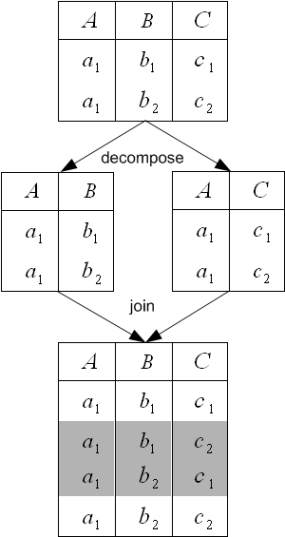
\includegraphics[scale=0.5]{./img/lossy01.png}
    \label{fig:lossy}
  }
  \subfigure[Lossless]{
    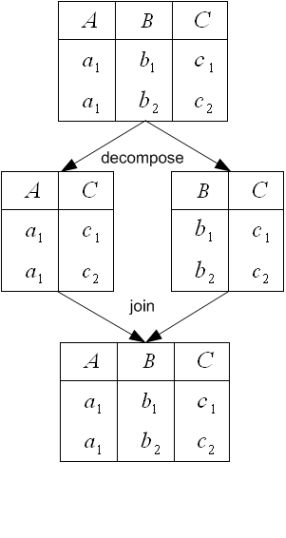
\includegraphics[scale=0.5]{./img/lossless01.png}
    \label{fig:lossless}
  }
\caption{Lossless-Join Property Example}
\end{figure}

\subsubsection{Dependency-Preservation Property}
Another desirable property in database design is dependency preservation. 
Let $F$ be a set of FDs that hold in $R$, which is decomposed into relations $R_1 ,..., R_n$.
Let $F_i$ denote (a cover of) $F\sp{+}$ consisting of those FDs whose LHS
and RHS both are contained in $R_i$. Then the decomposition is
dependency preserving if the following condition is satisfied: 
\begin{displaymath}
F \equiv (F_1 \cup ... \cup F_n ) \mbox{  respectively  } F\sp{+} = (F_1 \cup ... \cup F_n )\sp{+}
\end{displaymath}

In the following we illustrate the concept of dependency preservation with an example
of a decomposition which is does not satisfy this property: \\ \\
\indent $R = \{A, B, C, D\}$ \\
\indent $F = \{ABC \rightarrow D, D \rightarrow AB\}$ \\
\indent Decompose $R$ in: \\
\indent \begin{tabular}[h]{l l}
  $R_1 = \{C, D\}$  & $F_1 = \{ \}$ \\
  $R_2 = \{A,B,D\}$ & $F_2 = \{D \rightarrow AB \}$ \\
\end{tabular} \\

The decomposition is lossless-join, since $D \rightarrow ABD \in F\sp{+}$. However, 
the decomposition is \textbf{not} dependency preserving, because the FD $ABC \rightarrow D \in F\sp{+}$ but it is
not present in $(F_1 \cup F_2)\sp{+}$.

\section{Brief Introduction to the Normal Forms}
\label{sec:nfintro}
In the previous section we discussed some aspects on how to decompose a relation correctly, 
in this section we will continue this discussion by introducing some of the normal forms
namely the First Normal Form (1NF), Second Normal Form (2NF), Third Normal Form (3NF) and
Boyce-Codd Normal Form (BCNF). Normal forms are employed to avoid or eliminate 
the three types of data anomalies 
(insertion, deletion and update anomalies) which a database may suffer from. 
These concepts are clarified in the next section, after that we
define the different normal forms.

\subsection{Data Anomalies}
A relation that is not sufficiently normalized can suffer from logical inconsistencies of various types
called data anomalies. We illustrate the different data anomalies by
giving an example of a relation which suffers from all three anomalies: Insertion, Update and
Delete Anomaly. Figure~\ref{fig:relsc1nf}
shows the relation \textit{Student Courses}, which stores data about a student and the courses 
that he/she has taken. In addition, each student is assigned a mentor, who is 
a professor from the student's department. 

%\bgroup
%\setlength\LTleft{-2cm}\setlength\LTright{-2cm}%
%\LTXtable{\textwidth}{./tex/relation-sc.tex}
%\egroup

%\begin{sidewaystable}
%\begin{figure}[h]
%  \begin{center}
%    \begin{longtable}{|C|c|c|c|c|c|c|c|c|C|}
  \hline
  \multicolumn{10}{|c|}{\textit{Student Courses}} \\ \hline 
  \textbf{Matrl.} & Surname & Date of    & Mentor & Mentor  & Mentor   & \textbf{Course} & Course    & ECTS    & Grade \\* 
  \textbf{Nr.}    &         & Birth      & ID     & Surname & Office   & \textbf{Code}   & Name      & Credits &       \\ 
  \hline \hline
  100 & John     & 1976-09-28 & 101 & Codd   & B707 & 5DV001 & Database    & 7.5 & A \\ 
      &          &            &     &        &      &        & Concepts    &     &   \\ \hline
  100 & John     & 1976-09-28 & 101 & Codd   & B707 & 5DV002 & Operating   & 7.5 & B \\
      &          &            &     &        &      &        & Systems     &     &   \\ \hline
  200 & Schmidt  & 1986-05-19 & 201 & Turing & A612 & 5DV001 & Database    & 7.5 & B \\
      &          &            &     &        &      &        & Concepts    &     &   \\ \hline
  200 & Schmidt  & 1986-05-19 & 201 & Turing & A612 & 5DV002 & Operating   & 7.5 & B \\
      &          &            &     &        &      &        & Systems     &     &   \\ \hline
  200 & Schmidt  & 1986-05-19 & 201 & Turing & A612 & 5DV003 & Computer    & 7.5 & C \\
      &          &            &     &        &      &        & Networks    &     &   \\ \hline
  300 & Eriksson & 1984-02-29 & 101 & Codd   & B707 & 5DV004 & Distributed & 7.5 & A \\ 
      &          &            &     &        &      &        & Systems     &     &   \\ \hline
\end{longtable}
%    \caption{Relation Student Courses}
%    \label{fig:relsc1nf}
%  \end{center}
%\end{figure}
%\end{sidewaystable}

\begin{sidewaysfigure}
\begin{center}
\begin{longtable}{|C|c|c|c|c|c|c|c|c|C|}
  \hline
  \multicolumn{10}{|c|}{\textit{Student Courses}} \\ \hline 
  \textbf{Matrl.} & Surname & Date of    & Mentor & Mentor  & Mentor   & \textbf{Course} & Course    & ECTS    & Grade \\* 
  \textbf{Nr.}    &         & Birth      & ID     & Surname & Office   & \textbf{Code}   & Name      & Credits &       \\ 
  \hline \hline
  100 & John     & 1976-09-28 & 101 & Codd   & B707 & 5DV001 & Database    & 7.5 & A \\ 
      &          &            &     &        &      &        & Concepts    &     &   \\ \hline
  100 & John     & 1976-09-28 & 101 & Codd   & B707 & 5DV002 & Operating   & 7.5 & B \\
      &          &            &     &        &      &        & Systems     &     &   \\ \hline
  200 & Schmidt  & 1986-05-19 & 201 & Turing & A612 & 5DV001 & Database    & 7.5 & B \\
      &          &            &     &        &      &        & Concepts    &     &   \\ \hline
  200 & Schmidt  & 1986-05-19 & 201 & Turing & A612 & 5DV002 & Operating   & 7.5 & B \\
      &          &            &     &        &      &        & Systems     &     &   \\ \hline
  200 & Schmidt  & 1986-05-19 & 201 & Turing & A612 & 5DV003 & Computer    & 7.5 & C \\
      &          &            &     &        &      &        & Networks    &     &   \\ \hline
  300 & Eriksson & 1984-02-29 & 101 & Codd   & B707 & 5DV004 & Distributed & 7.5 & A \\ 
      &          &            &     &        &      &        & Systems     &     &   \\ \hline
\end{longtable}
\caption{Relation Student Courses}\label{fig:relsc1nf}
\end{center}
\end{sidewaysfigure}

\begin{description}
  \item[Insertion Anomaly] means that that some data can not be 
    inserted in the database. For example we can not add a new course to the \textit{Student Courses}
    relation, unless we insert a student who has taken that course.
  \item[Update Anomaly] means we have data redundancy in the database and to make any 
    modification we have to change all copies of the redundant data or else the 
    database will contain incorrect data. For example in our database we have the course 
    \textit{Database Concepts} which appears in several tuples in our relation. 
    To change its description to \textit{New Database Concepts} we have to change 
    it in all tuples. Indeed, one of the purposes of normalization is to eliminate data 
    redundancy in the database.
  \item[Deletion Anomaly] means deleting some data cause other information to be lost. 
    For example, if the student Eriksson is deleted from the relation we also lose the 
    information that we had a course \textit{Distributed Systems}.
\end{description}

\subsection{First Normal Form} 
A relation is in first normal form (1NF) if each of
the domains of its attributes is simple or atomic. 
In other words, none of the attributes of the relation is a compositition of multiple attributes, 
a set of values nor a relation. The following relation is not in 1NF:

\begin{center}
\begin{tabular}[h]{|l|l|l|l|}
  \hline
  Matrl.Nr. & Surname & Date\_of\_Birth & Taken\_Courses \\ \hline
  100 & John & 1976-09-28 & \{Database Concepts, Operating Systems \} \\  
  200 & Schmidt & 1986-05-19 & \{Database Concepts, Operating Systems,  \\ 
      &         &            & Computer Networks \} \\
  300 & Eriksson & 1984-02-29 & \{Distributed Systems \} \\ \hline
\end{tabular}
\end{center}

The attribute \textit{Taken\_Courses} violates the 1NF rule, since it is a set of 
course names. To avoid this we can use a relation similar to the \textit{Student Courses} relation,
which is in 1NF. However, it was shown in the previous section that the relation suffers
from all three data anomalies, therefore we need further restrictions to the 1NF. We
introduce these in the following sections.  

\subsection{Second Normal From}
A relation is in 2NF if it is in 1NF and all its non-key attributes are fully
functionally dependent on every candidate key of the relation.
Note that key attributes are those attributes which are parts of any 
candidate key, and non-key attributes do not participate in any candidate key. 

The relation \textit{Student Courses} is not in 2NF. In order to prove this we must
first define a set of FDs on the relation. Figure~\ref{fig:fds01a} is a graphical representation 
of the FDs between the primary key \textit{\{Matrl.Nr., Course\_ID\}} and the rest of the 
attributes in the \textit{Student Courses} relation. 
Note that the attribute to the right of the arrow is functionally dependent on the attribute 
in the left of the arrow.  

\begin{figure}[h]
  \begin{center}
    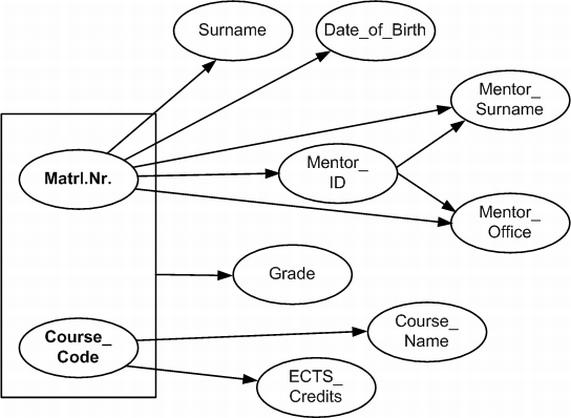
\includegraphics[width=0.6\textwidth]{./img/fds01b.png}
    \caption{Set of FDs which hold in Student Courses}
    \label{fig:fds01a}
  \end{center}
\end{figure}

As can be seen only the \textit{Grade} attribute is fully functionally dependent on the primary key.
On the other hand, the attributes \textit{Surname, Date\_of\_Birth, Mentor\_ID, Mentor\_Surname, Mentor\_Office, Course\_Name, ECTS\_Credits} 
and \textit{Grade} are all non-key attributes because none of them is a component of a candidate key, therefore
the relation is not in 2NF. 

To convert \textit{Student Courses} to 2NF we have to make all non-primary attributes 
be fully functionally dependent on the primary key. 
To do that we can decompose the \textit{Student Courses} relation into the following three new relations:
\textit{Student and Mentors = \{Matrl.Nr., Surname, Date\_of\_Birth, Mentor\_ID, Mentor\_Office, Mentor\_Surname\}}, 
\textit{Courses = \{Course\_ID, Course\_Name, ECTS\_Credits\}} and 
\textit{Grades = \{Matrl.Nr., Course\_ID,  Grade\}}.
Figure~\ref{alg:relsc2nf} shows these three relations and their contents.


\begin{figure}[h]
\hrule
\vspace{0.25cm}
\begin{center}
\begin{tabular}[h]{|c|c|c|c|c|c|}
\hline
\multicolumn{6}{|c|}{\textit{Students and Mentors}} \\ \hline
\textbf{Matrl.Nr.} & Surname & Date\_of\_  & Mentor\_ & Mentor\_  & Mentor\_ \\
                   &         & Birth       & ID       & Surname   & Office \\
 \hline \hline
 100 & John     & 1976-09-28 & 101 & Codd   & B707 \\
 200 & Schmidt  & 1986-05-19 & 201 & Turing & A612 \\
 300 & Eriksson & 1984-02-29 & 101 & Codd   & B707 \\ \hline
\end{tabular} 
\end{center}

\vspace{0.5cm}

\begin{minipage}[t]{0.5\linewidth}
\centering
\begin{tabular}[h]{|c|c|c|}
\hline
\multicolumn{3}{|c|}{\textit{Courses}} \\ \hline
\textbf{Course\_} & Course\_Name & ECTS\_ \\
\textbf{Code} &  & Credits \\
\hline \hline
5DV001 & Database Concepts   & 7.5 \\ 
5DV002 & Operating  Systems  & 7.5 \\
5DV003 & Computer  Networks  & 7.5 \\
5DV004 & Distributed Systems & 7.5 \\ \hline
\end{tabular}

\end{minipage}
\hspace{0.5cm}
\begin{minipage}[t]{0.5\linewidth}
\centering
\begin{tabular}[h]{|c|c|c|}
  \hline
  \multicolumn{3}{|c|}{\textit{Grades}} \\ \hline
  \textbf{Matrl.Nr.} & \textbf{Course\_} & Grade \\
   & \textbf{Code} &  \\
  \hline \hline
  100 & 5DV001 & A \\ 
  100 & 5DV002 & B \\
  200 & 5DV001 & B \\
  200 & 5DV002 & B \\
  200 & 5DV003 & C \\
  300 & 5DV004 & A \\ \hline
\end{tabular}
\end{minipage}

\caption{Decomposition of Relation Student Courses in 2NF}\label{alg:relsc2nf}
\hrule
\end{figure}

All three relations are in 2NF. Furthermore, it can be proven that the
decomposition is lossless-join and dependency preserving. 
Examination of the new relations shows that we have eliminated most of the redundancy 
in the database. The relations \textit{Courses} and \textit{Grades} are free
from any data anomalies. However, the \textit{Students~and Mentors} relation still suffers form all three
data anomalies, because it also keeps track of all mentors:
\begin{enumerate}
  \item We cannot add new mentors without adding new students.
  \item To change the office of a mentor we have to update several tuples.
  \item If the student Schmidt is deleted we also lose the information about the mentor Turing.
\end{enumerate}
 
\subsection{Third Normal Form}
A relation $R$ is in 3NF if it is in 2NF and for all FDs that hold in $R$
of the form $\alpha \rightarrow B$, where $\alpha \subseteq  R$ and $B \in R$, 
at least one of the following holds: 
\begin{enumerate}
  \item $B \in \alpha$, i.e., the FD is trivial
  \item $B$ is a prime attribute, i.e., $B$ is part of a candidate key.
  \item $\alpha$ is a superkey of $R$.
\end{enumerate}

From the three previous relations only \textit{Students and Mentors} is not in 3NF, since 
the FD \textit{Mentor~ID $\rightarrow$ Mentor~Surname, Mentor~Office} holds in the relation but 
it violates the 3NF property. Therefore we need to further decompose the relation into two
new relation: \textit{Students~= \{Matrl.Nr., Surname, Date\_of\_Birth, Mentor\_ID\}} and
\textit{Mentors~= \{Mentor\_ID, Mentor\_Surname, Mentor\_Office\}}.
Figure~\ref{alg:relsc3nf} shows the two new relations and their content.

\begin{figure}[h]
\hrule
\vspace{0.25cm}
\begin{minipage}[t]{0.5\linewidth}\centering
\begin{tabular}{|c|c|c|c|}
\hline
\multicolumn{4}{|c|}{\textit{Students}} \\
\hline
\textbf{Matrl.Nr.} & Surname & Date\_of\_  & Mentor\_ \\
                   &         & Birth    & ID\_     \\
\hline \hline
100 & John     & 1976-09-28 & 101 \\
200 & Schmidt  & 1986-05-19 & 202 \\
300 & Eriksson & 1984-02-29 & 101 \\
\hline
\end{tabular}
\end{minipage}
\hspace{0.5cm}
\begin{minipage}[t]{0.5\linewidth}\centering
\begin{tabular}{|c|c|c|}
\hline
\multicolumn{3}{|c|}{\textit{Mentors}} \\ \hline
 \textbf{Mentor\_} & Mentor\_  & Mentor\_ \\
 \textbf{ID}       & Surname   & Office \\
 \hline \hline
 101 & Codd   & B707 \\
 201 & Turing & A612 \\ \hline
\end{tabular}
\end{minipage}

\caption{Decomposition of Relation Students and Mentors in 3NF}\label{alg:relsc3nf}
\hrule
\end{figure}

It can be shown that the two new relations are in 3NF. Furthermore, the 
decomposition has the lossless-join and dependency-preserving properties. Indeed, it is always 
possible to find a dependency-preserving, lossless-join decomposition which is in 3NF~\cite[Section 6.8]{bdb2}.
However, a 3NF decomposition does not necessarily satisfy these properties. Consider the following example
of a 3NF decomposition which is not dependency preserving:

\begin{center}
\begin{tabular}[h]{l l}
  $R = \{A, B, C, D\}$ & $F = \{A \rightarrow BC, C \rightarrow D, D \rightarrow B\}$ \\
  Decompose $R$ in:  & $R_1 = \{A, B, C\} \mbox{ and } R_2 = \{C,D\}$ \\ 
\end{tabular}
\end{center}

Returning to the running example, it is worth noting that our original relation \textit{Student Courses} is now decomposed
into four different relations: \textit{Students, Mentors, Courses} and \textit{Grades}. The 
decomposition is in 3NF, this means that each member of the set of relation schemes is in 3NF. 
More importantly, the decomposition does not suffer any data anomalies. 
Let us clarify this in more detail:
\begin{description}
  \item[Insertion Anomaly:] Now new mentors and courses can be inserted to the relation \textit{Mentors}/\textit{Courses} without needing to add new students.
  \item[Update Anomaly:] Since redundancy of the data was eliminated no update anomaly can occur. For example, to change the \textit{Course Name} for 5DV001 only one change is needed in the relation \textit{Courses}.
  \item[Deletion Anomaly:]  The deletion of student Schmidt from the database is achieved by deleting Schmidt's records from both \textit{Students} and \textit{Grades} relations and this does not have any side effects on the different courses or mentors, since they stay untouched in their own relations.  
\end{description}

\subsection{Boyce-Codd Normal Form}
\label{sec:BCNF}
BCNF is a slightly stronger than 3NF. A relation scheme $R$ is in BCNF 
with respect to a set $F$ of FDs if $R$ is in 3NF and for all functional dependencies in $F\sp{+}$ 
of the form $\alpha \rightarrow \beta$, where $\alpha \subseteq R$ and $\beta \subseteq R$,
at least one of the following holds:
\begin{enumerate}
  \item $\alpha \rightarrow \beta$ is a trivial functional dependency (i.e. $\beta \subseteq \alpha$)
  \item $\alpha$ is a superkey for $R$ 
\end{enumerate}

Only in rare cases a 3NF relation does not meet the requirements of BCNF. In fact, our decomposition 
\textit{\{Students, Mentors, Courses, Grades\}} is in BCNF. Let us consider the following
example of a relation which is in 3NF but not in BCNF.  The example 
comes from~\cite[Section 6.5.3]{bdb2}.

\begin{center}
\begin{tabular}[h]{l l}
  $PostalCodeIndex = \{Street, City, Province, PostalCode\}$ & \\ [0.5ex]
  $F = \{Street, City, Province \rightarrow PostalCode; \mbox{ } PostalCode \rightarrow City, Province\}$ \\ [1.5ex]
  The FD $PostalCode \rightarrow City, Province$ is not trivial and it is not a superkey, \\ [0.5ex]
  thus the $PostalCodeIndex$ relation is not in BCNF. & \\ [1.5ex]
  BCNF decomposition of $PostalCodeIndex$:   &  \\ [0.5ex]
  $Streets =\{PostalCode, Street\}$ & \\ [0.5ex]
  $Cities = \{PostalCode, City, Province\}$ & \\ [0.5ex]
\end{tabular}
\end{center}

The decomposition \textit{\{Streets, Cities\}} is lossless-join, but it is not dependency-preserving. 
Indeed, some schemata do not have dependency-preserving decompositions
into BCNF, as such they are considered pathological by some.
